\documentclass[11pt,letter]{article}
\usepackage{amssymb}
\usepackage{amsmath}
\usepackage{graphicx}
\usepackage{enumerate}
\usepackage{epstopdf}
\usepackage{eucal}
\usepackage{listings}
\usepackage{color}

\definecolor{dkgreen}{rgb}{0,0.6,0}
\definecolor{gray}{rgb}{0.5,0.5,0.5}
\definecolor{mauve}{rgb}{0.58,0,0.82}

\addtolength{\oddsidemargin}{-.75in}
\addtolength{\evensidemargin}{-.75in}
\addtolength{\textwidth}{1.5in}
\addtolength{\topmargin}{-.75in}
\addtolength{\textheight}{1.5in}
\setlength{\parindent}{0pt}
\def\bnabla{\mbox{\boldmath$\nabla$}}
\usepackage{subfigure}

\begin{document}
\begin{center}
	\large\textbf{Optimizing Interventions in the Ebola Epidemic Using a Compartmental Model}\\
	\normalsize{Final Report\\APC 524, Fall 2014}
\end{center}

\underline{\textbf{Developers}}\vspace{0.5mm}\\Jesse Ault\\Alta Fang\\Sandra Sowah\\ Yile Gu\\

\underline{\textbf{Project Objective}}\vspace{0.5mm}\\
The software package we present here determines how to optimally allocate a given, finite number of resources during an Ebola virus outbreak in order to minimize the spread of the disease and contain the outbreak. This software package uses a stochastic compartmental model~[1] to simulate the spread of the disease. Given resource constraints and epidemic information, it fits the model parameters to the epidemic data and uses that model to forecast the effect of certain interventions on the trajectory of the disease. By modeling the effects of different intervention distributions, the software determines how a fixed quantity of resources can be allocated in order to minimize the total number of deaths due to the Ebola epidemic.\\

\underline{\textbf{Package Overview}}\vspace{0.5mm}\\
Our software package allows users to interact through either a friendly python command interface or a GUI interface. The user can provide 1) a time series of cumulative Ebola infection case counts in a comma-separated values (csv) file, 2) the total population of the corresponding region, and 3) the total resources and cost functions for each intervention in an additional csv file. Using these inputs, the program can calculate the compartmental model parameters, the optimal resource allocation, and projections of the spread of Ebola with or without the interventions applied. The software can visualize the projected outbreak for the case with no interventions, the case with user-specified interventions, and the case with the calculated optimum interventions. The user has the option to generate figures to inspect the quality of the model fit to the original case counts data, as well as the projected time series of the disease spread. Installation is needed in order to fully utilize the code. For installation details, please refer to the user manual.\\

\underline{\textbf{Compartmental Model Overview}}\vspace{0.5mm}\\
A compartmental model [1-2] has been proposed and used to study the Ebola outbreaks in the Democratic Republic of Congo (1995), in Uganda (2000), and in Sierra Leone and Liberia (2014). In this compartmental model, individuals are classified as: (1) susceptible individuals, S, who can be infected by the Ebola virus following contact with infectious cases; (2) exposed individuals, E, who have been infected by the Ebola virus but are not yet infectious or symptomatic; (3) symptomatic and infectious individuals in the community, I; (4) hospitalized Ebola cases, H, who are infectious; (5) dead Ebola cases, F, who may transmit the disease during funeral procedures; and (6) individuals removed from the chain of transmission, R, due to recovering from the disease or being buried. The dynamics for the population of these types of individuals are modeled through the coupled ordinary differential equations (ODEs) given in the following system:
\begin{subequations}
	\begin{align}
		&\frac{dS}{dt}=-\frac{1}{N}\left(\beta_ISI+\beta_HSH+\beta_FSF\right),\\
		&\frac{dE}{dt}=\frac{1}{N}\left(\beta_ISI+\beta_HSH+\beta_FSF\right)-\alpha E,\\
		&\frac{dI}{dt}=\alpha E-\left(\gamma_h\theta_1+\gamma_i(1-\theta_1)(1-\delta_1)+\gamma_d(1-\theta_1)\delta_1\right)I,\\
		&\frac{dH}{dt}=\gamma_h\theta_1I-\left(\gamma_{dh}\delta_2+\gamma_{ih}(1-\delta_2)\right)H,\\
		&\frac{dF}{dt}=\gamma_d(1-\theta_1)\delta_1I+\gamma_{dh}\delta_2H-\gamma_fF,\\
		&\frac{dR}{dt}=\gamma_i(1-\theta_1)(1-\delta_1)I+\gamma_{ih}(1-\delta_2)H+\gamma_fF.
	\end{align}
	\label{eq:ODEs}
\end{subequations}

\vspace{-3mm}These governing ODEs consider the populations of each compartment to be continuous. Solving this type of system is deterministic. A given solution can be found for given inputs. However, we know that the populations are not continuous. Instead, they are always discrete, and they are always integers. Thus, while a deterministic formulation of the problem may result in a solution that represents the most probable outcome, we know that many outcomes are actually possible. Thus, for this type of problem a stochastic formulation of the equations can be more appropriate. With this approach, the interpretation of the coefficients in equations \ref{eq:ODEs} is changed. In the deterministic formulation, these coefficients are thought of as reaction ``rates.'' However, in the stochastic formulation they are interpreted as reaction ``probabilities per unit time.'' Using a stochastic formulation, we can solve for not only the most probable outcome of the outbreak, but we can also solve for standard deviations and confidence intervals to understand the worst- and best- case scenarios. In order to solve the stochastic formulation of the basic equations (\ref{eq:ODEs}), we utilize Gillespie's first reaction method [3]. In order to solve for a single trajectory for the future compartmental values, the Gillespie algorithm can be briefly summarized as follows:
\begin{enumerate}
	\item{Initialize the compartment populations and reaction constants.}
	\item{For each possible reaction (infection, death, hospitalization, etc...), calculate the probability that it will be the next reaction.}
	\item{Generate random numbers to determine the next reaction using the probabilities and the time interval to next reaction.}
	\item{Update and repeat until the final time.}
\end{enumerate}
For more details, see [3]. Using these steps, a single trajectory is solved for. By generating many trajectories, mean trajectories and standard deviations can be generated with increasing accuracy as the number of trajectories is increased. Thus, this solution algorithm may be effectively thought of as a dynamic Monte Carlo method.\\

\underline{\textbf{Model Parameters and Interventions}}\vspace{0.5mm}\\
The governing ODEs contain many parameters and rate constants. These are summarized in Table~1. For our stochastic formulation, we interpret the rate constants $\beta_I$, $\beta_H$, and $\beta_F$ as probabilities that a an individual will become infected in the community, in a hospital, and at a funeral, respectively, in a certain time interval.

\begin{table}
\caption{Summary of relevant parameters from the governing ODEs}
\begin{center}
\begin{tabular}{|c|c|}
\hline
\textbf{Parameter}&\textbf{Meaning}\\
\hline
N&Total population\\
\hline
$\beta_I$&Transmission rate in the community\\
\hline
$\beta_H$&Transmission rate after hospitalization\\
\hline
$\beta_F$&Transmission rate during traditional burial\\
\hline
$1/\alpha$&Mean duration of the incubation period\\
\hline
$1/\gamma_h$&Mean duration between onset of symptoms and hospitalization\\
\hline
$1/\gamma_i$&Mean duration of the infectious period for survivors\\
\hline
$1/\gamma_d$&Mean duration of the infectious period for patients who died\\
\hline
$1/\gamma_f$&Mean duration of the infectious period between death and burial\\
\hline
$1/\gamma_{dh}$&Mean duration from hospitalization to death\\
\hline
$1/\gamma_{ih}$&Mean duration from hospitalization to end of infectious period\\
\hline
$\theta$&Percent of cases hospitalized\\
\hline
$\delta$&Case-fatality ratio\\
\hline
\end{tabular}
\end{center}
\end{table}

In addition, $\theta_1$, $\delta_1$, and $\delta_2$ are given by
\begin{subequations}
	\begin{align}
		&\theta_1=\frac{\theta[\gamma_i(1-\delta_1)+\gamma_d\delta_1]}{\theta[\gamma_i(1-\delta_1)+\gamma_d\delta_1]+(1-\theta)\gamma_h},\\
		&\delta_1=\frac{\delta\gamma_i}{\delta\gamma_i+(1-\delta)\gamma_d},\\
		&\delta_2=\frac{\delta\gamma_{ih}}{\delta\gamma_{ih}+(1-\delta)\gamma_{dh}}.
	\end{align}
\end{subequations}

In order to perform our interventions study, we first determine which parameters may be affected through interventions. We recognize three parameters that could possibly be affected through the use of interventions. First, the transmission rate at hospitals may be reduced by purchasing personal protective equipment and other supplies. Secondly, investing in drugs and treatments may reduce the fatality rate of hospitalized patients. Finally, through contact tracing and community awareness a larger percentage of those infected can be taken to the hospital. These are selected as our intervention parameters and summarized in Table 2. Note that, in some cases, specific combinations of interventions can actually increase the total number of deaths. For example, if a country has very poor quality hospitals with minimal protective equipment and a low survival rate, then allocating all resources to hospitalizing the infected can actually accelerate the number of deaths, as they may have a lower chance of survival in an unsanitary hospital.\\

\begin{table}
\caption{Intervention parameters}
\begin{center}
\centering
\begin{tabular}{|c|c|c|}
\hline
\textbf{Parameter} & \textbf{Intervention}                                                                       & \textbf{Effect}                                                                                  \\ \hline
$\beta_H$          & \begin{tabular}[c]{@{}c@{}}Personal protective equipment\\  and other supplies\end{tabular} & \begin{tabular}[c]{@{}c@{}}Contact rate for \\ hospitalized cases\end{tabular}                   \\ \hline
$\delta_2$         & Hypothetical drug                                                                           & \begin{tabular}[c]{@{}c@{}}Fatality rate of \\ hospitalized patients\end{tabular}                \\ \hline
$\theta_1$         & \begin{tabular}[c]{@{}c@{}}Contact tracing and \\ community awareness\end{tabular}          & \begin{tabular}[c]{@{}c@{}}Fraction of infected \\ cases diagnosed and hospitalized\end{tabular} \\ \hline
\end{tabular}
\label{para}
\end{center}
\end{table}

One of the largest uncertainties in our resource allocation comes from assigning cost functions to our resources. For example, how can a given amount of personal protective equipment affect the probability that someone will become infected in the hospital. Such a specific relationship would be difficult to find in practice apart from experimental data. Such data would need to be specific to each country, and furthermore specific to the current socio-economic state of the country. In general, such data is not available, and so we assume specific relationships for our cost function with the hope and understanding that with the right information these software tools could provide even more accurate results. We assume that $\beta_H$ and $\delta_2$ increase and $\theta_1$ decreases linearly as the resources allocated to each of them increases. For example, if we give $x$ amount of resources to purchasing personal protective equipment for hospitals, then $\beta_H$ will decrease by a given amount $y$. If instead we gave $2x$, then $\beta_H$ would decrease by $2y$. Thus, given a fixed quantity of resources, we determine how to most efficiently allocate those resources among these three interventions. This is done by incorporating the epidemic model into an optimization cost function and performing constrained optimization to calculate the most efficient resource allocation that will minimize the expected number of deaths.\\

Thus, we minimize a cost function $f(x_1,x_2,x_3)$ representing the calculated average number of deaths over a given number of trajectories, subject to the constraints that 
\begin{equation}
\sum\limits_{1}^{3}x_i=1\text{~~~~and~~~~}x_i>0,
\end{equation} 
where $x_i$ represents the fraction of total resource allocated to each of the three interventions. \\

\underline{\textbf{Software Tools}}\vspace{-0.5mm}\\
Throughout the design process, we attempted to select the appropriate software tools for us to meet our design goals. Luckily, many powerful tools were introduced during the semester. Since we desired to use Python for our main code in order to generate a user-friendly interface, the obvious choices for us to use for visualization/plotting, optimization, distribution, and testing were Matplotlib, Scipy, Distutils, and Unittest, respectively. One of our members had a background in using Sphinx for documentation, and so we selected to use that for our software package. Git was selected for our version control since several of us had experience with it. OpenMP was selected for parallelization because we wanted to be able to run on a single processor. Since none of the members of our team had any experience interfacing C++ and Python code, Cython was selected because it appeared to be the most common tool for the job. Finally cProfile was used to profile the code for its ease of use. These design tools are summarized in Table 3.\\

\begin{table}
\caption{Software tools used in this project}
\begin{center}
	\begin{tabular}{ |l|l| }
	\hline
	\textbf{Purpose} & \textbf{Software Tool} \\ 
	\hline
	Visualization/Plotting & Matplotlib \\
	\hline
	Optimization & Scipy \\
	\hline
	Documentation  & Sphinx \\
	\hline
	Distribution & Distutils \\
        \hline
        Testing  & Python Unittest \\
        \hline
        Interfacing C++ and Python & Cython \\
        \hline
        Parallelization & OpenMP \\
        \hline
        Version Control & Git \\
        \hline
        Profiling & cProfile \\ 
        \hline
        Graphical User Interface & PyQt \\
        \hline
	\end{tabular}
\end{center}
\end{table}

\underline{\textbf{Design Process and Software Overview}}\vspace{0.5mm}\\
We initially identified four primary, independent goals for our software package:
\begin{enumerate}
	\item{Solve the stochastic rate equations and return the projected future cases as well as the total number of deaths.}
	\item{Read in the user-supplied outbreak data and find the optimum parameters that minimize the fit between the ODEs and the data.}
	\item{Provide a simple, powerful interface for the user which can call the stochastic solver using the determined best-fit parameters and minimize the total number of deaths, optimizing the resource allocation.}
	\item{Interpret the results and communicate them to the user.}
\end{enumerate}
These natural divisions in the software served as our initial division of labor (apart from design documents, reports, and presentations).\\

At the heart of the code is the stochastic equation solver which actually calculates the future time data series projections, standard deviations, and total deaths. StochPy [4] is a ``comprehensive, user-friendly tool for simulating stochastic biological processes.'' This freely-available software is described as accessible, functional, and flexibly. We initially thought that StochPy could be a valuable tool. Since it is written in Python, we expected that our code could easily interface with it. Furthermore, the flexibility of StochPy allowed us to easily implement our compartmental model. However, some basic profiling with a stopwatch quickly showed us that StochPy was much too slow for our purposes. Generally speaking, hundreds of trajectories are needed to achieve reliable average time series projections as well as accurate standard deviations. Furthermore, with an outer loop optimization, we can expect to run those hundreds of trajectories at least tens of times. However, with a single set of parameters, StochPy took over 1000 seconds to solve for just 24 trajectories. Thus, we could expect the software to take hours, or even days, to solve an optimization loop with $\mathcal{O}$(100) trajectories.\\

Thus, we sought an alternative to StochPy that would: a) be much faster, and b) be simpler to interface with our Python code. This led us to implement our own stochastic equation solver, StochCalc, in C++, using Cython to manage the interface with our Python code. After a serial version of StochCalc was implemented, along with a simple interface, profiling demonstrated significant speedups relative to the StochPy solver, which will be described below. Furthermore, we also realized that the stochastic solver was an ideal candidate for parallelization, since each trajectory is independent of the others. Thus, without changing the interface, the implementation of StochCalc was parallelized using OpenMP, resulting in further speed increases.\\

To find the optimum parameters that give the best fit, we used the optimization package in Scipy. There are many different minimization methods provided, and we chose COBYLA because it allows for the inclusion of constraints. For constraints used here, consistent with the previous literature [1-2], all the parameters need to be positive and the ones representing fractions need to be smaller than 1. \\

The resource allocation optimization code structure was designed to be as modular as possible, since it required interfacing with model fitting, stochastic simulations, and output plotting. Scipy was used since it was a standard and easy-to-use tool to solve optimization problems, with an interface that allowed easy switching between different algorithms to tackle the same problem. Inspiration for our software's optimization wrapping was drawn from Mystic, a python optimization software package (https://github.com/uqfoundation/mystic) that one of us previously contributed to developing. However, we opted not to actually use Mystic to do our optimization in order to reduce the number of dependences of our software package and because Mystic's handling of constrained optimization did not seem to be sufficiently robust and well-developed. \\

After successfully interfacing all of the software components of our software together, the software package may be visualized using the Unified Modeling Language (UML). This is shown in figure~\ref{fig:UML}.
\begin{figure}
\centering
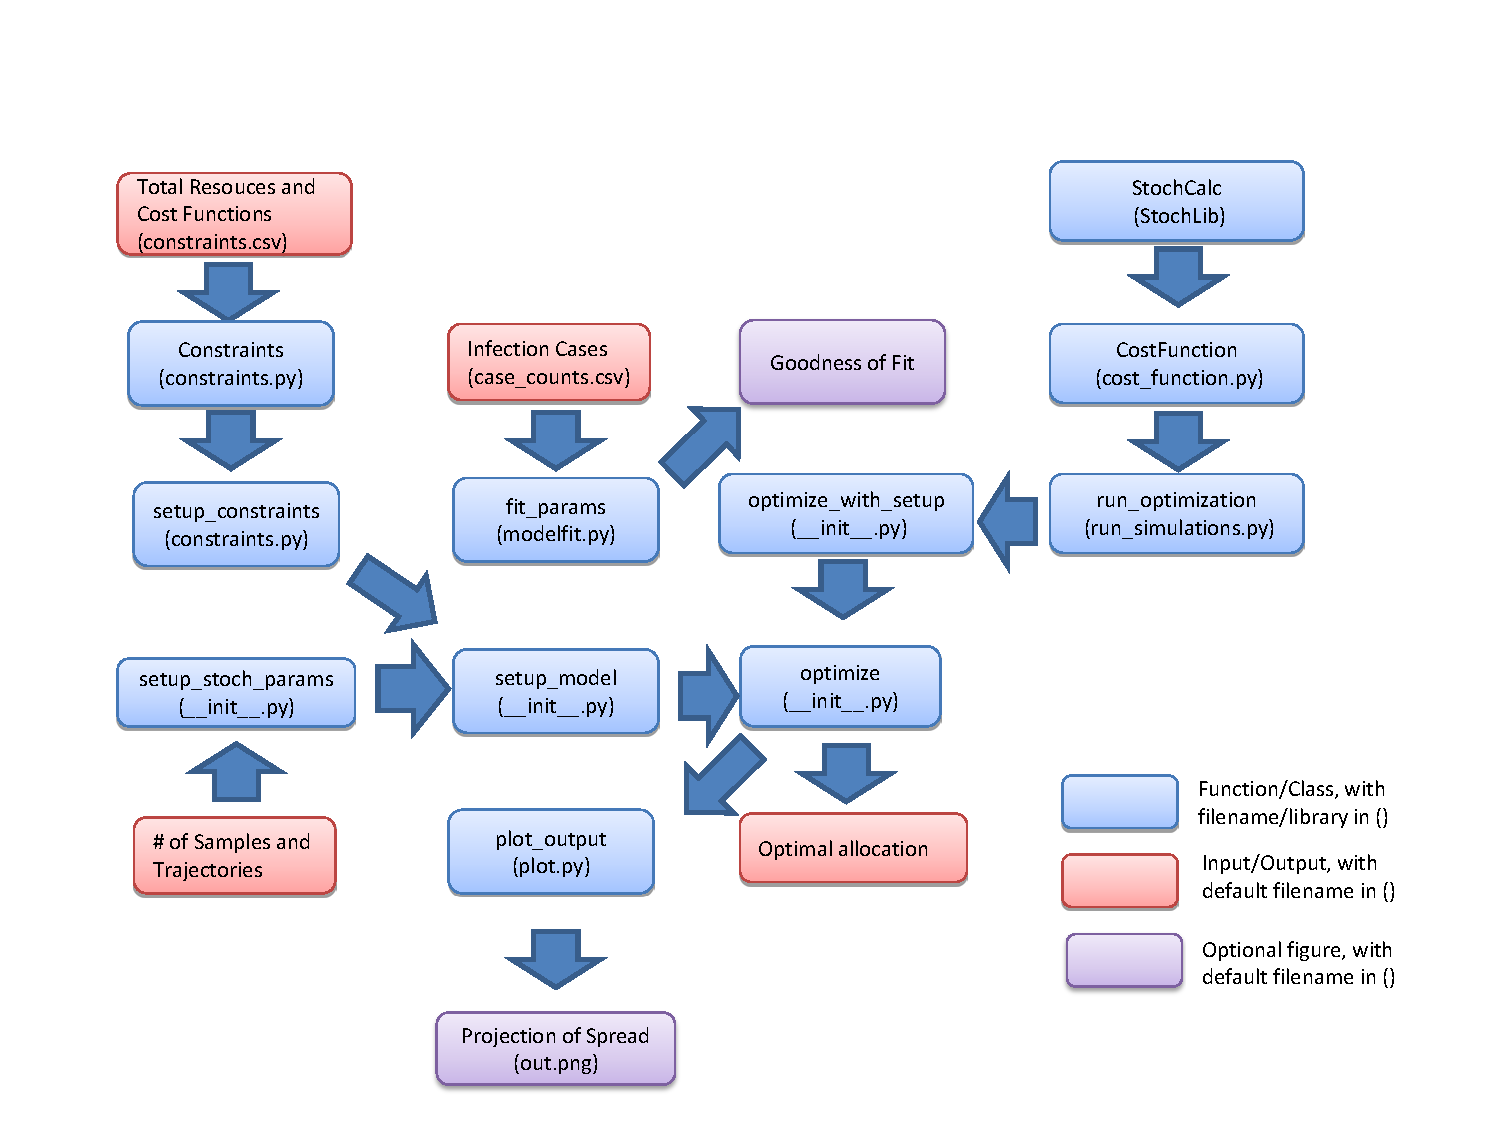
\includegraphics[width=16cm]{Design_FlowChart.pdf}
\caption{Unified Modeling Language of our software package}
\label{fig:UML}
\end{figure}

\underline{\textbf{Software Package: Main Functions}}\\

{\textbf{fit\_params}}\vspace{3mm}\\
\hangindent=1cm{\textbf{Functionality:} The function fit\_params reads in the time series data of the infection cases and outputs the best fit model parameters. It can also optionally output a figure comparing the compartmental model to the data.\vspace{3mm}\\
\textbf{Specifics:} The deterministic formulation of the compartmental model is implemented as a function named SIRode. The initial guess for the model parameters are initialized using values from the literature [2]. The Constrained Optimization BY Linear Approximation (COBYLA) method from SciPy is used to minimize the difference between the model predictions and the data, with appropriate constraints on the model parameters. The model parameters are stored in a pyModelParams class which is a Cython container class for passing the model parameters to the StochCalc C++ solver.}\\

{\textbf{StochCalc}}\vspace{3mm}\\
\hangindent=1cm{\textbf{Functionality:} The function StochCalc is our C++ stochastic equation solver for the compartmental model [1]. StochCalc accepts as inputs a StochParams object which contains the parameters for the solver, a ModelParams object which contains the parameters for the model, another ModelParams object which contains the intervention parameters, the time to apply interventions, an optional output file name, and the number of OpenMP threads to use. The function returns the total number of deaths.\vspace{3mm}\\
\textbf{Specifics:} ModelParams and StochParams are two C++ container classes which group together the parameters relevant to the model (e.g. rate coefficients, etc...) and parameters relevant to the stochastic solver (e.g. initial compartment populations, etc...), respectively. They have Cython equivalent classes defined in StochLib.pyx which defines the interface between the Python and C++ code. StochCalc uses OpenMP to parallelize the stochastic solver across the number of trajectories.}\\

{\textbf{run\_optimization}}\vspace{3mm}\\
\hangindent=1cm{\textbf{Functionality:} The run\_optimization function uses the model parameter values calculated by the fit\_params function and calls the StochCalc function to determine the total number of expected deaths. Using an optimization loop, it finds the optimal resource allocation for minimizing the total number of deaths. \vspace{3mm}\\
\textbf{Specifics:} The COBYLA method from SciPy is once again used for minimization. The function to be minimized is represented by a CostFunction callable object that calls StochCalc for calculations and is initialized using parameters from fit\_params as well as user input. To prevent unreasonable results, two tests are performed before the optimization. Specifically, the intervention time is checked to make sure it is less than the final time of the simulation. Also, the total resource budget is checked to ensure that all of the interventions will not be maximized. In either of those cases, no optimization is be necessary, and only one simulation is performed.}\\

\underline{\textbf{Testing}}\\
Unitest has been used throughout our software design process to test our python scripts. Test files are located in the \emph{ebolaopt/tests} folder. \\

\textbf{test\_modelfit.py:} This test suite is used to test the fit\_params function.\vspace{3mm}\\
\hangindent=1cm{\textbf{Test 1:} Does the code give reasonable results for different countries?\vspace{3mm}\\
\textbf{Test 2:} Can the code optionally output figures comparing the model predictions with the history data?\\
}

\textbf{test\_optimization.py:} \hangindent=1cm{This test suite is used to test the resource allocations functions, including run\_optimization.\vspace{3mm}\\
\textbf{Test 1:} Does the optimization correctly stop if the intervention time is greater than the final time?\vspace{3mm}\\
\textbf{Test 2:} Does the optimization correctly stop if the total resources are too large?\vspace{3mm}\\
\textbf{Test 3:} Does the optimization work correctly for different countries?\vspace{3mm}\\
\textbf{Test 4:} Does the optimization still work when all resources are allocated to one intervention?\vspace{3mm}\\
\textbf{Test 5:} Does the optimization still work when the StochCalc solver is used in parallel?\vspace{3mm}\\
\textbf{Test 6:} Does the optimization actually return better results than non-optimal resource allocation cases? More details about the results from this test are include in the Simulation Results and Discussion section.\vspace{3mm}\\
\textbf{Test 7:} Does the ``valid\_interventions'' keyword work as expected?
}\\

\textbf{test\_stochcalc.py:} \hangindent=1cm{This test suite is used to test the StochCalc solver and Cython interface.\vspace{3mm}\\
\textbf{Test 1:} Does the StochCalc solver run without interventions?\vspace{3mm}\\
\textbf{Test 2:} Does the StochCalc solver run with interventions?\vspace{3mm}\\
\textbf{Test 3:} Does applying interventions actually decrease the number of deaths?\vspace{3mm}\\
\textbf{Test 4:} Does the StochCalc solver successfully run in parallel with 4 threads?\vspace{3mm}\\
\textbf{Test 5:} Does progressively delaying the start of interventions increase the number of deaths?\vspace{3mm}\\
\textbf{Test 6:} Does the code experience a speedup when run in parallel?
}\\

\underline{\textbf{Testing: StochPy vs. StochCalc}}\\
In addition to testing the functionality of our software package, we also need to ensure that it returns reasonable results. This is difficult, because there are no standard solutions that we can compare our results against. So, we instead simulate the same case using our StochCalc solver and compare the results to results generated by the StochPy solver. We assume that the StochPy solver gives true results. A comparison between the results generated by the two solvers is shown in figure \ref{StochPyComparison}.\\

\begin{figure}
	\centering
	\subfigure[]{
	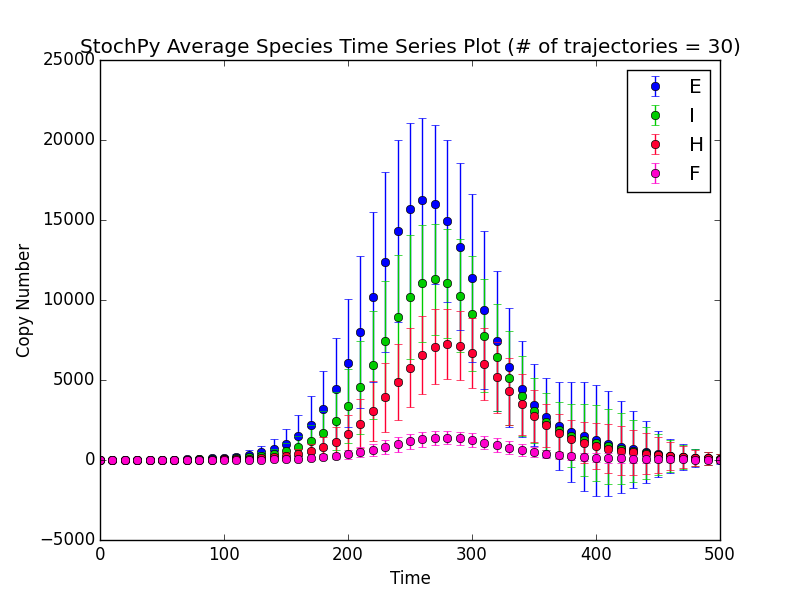
\includegraphics[width = 3.165 in]{StochPyEIHF.png}}
	\subfigure[]{
	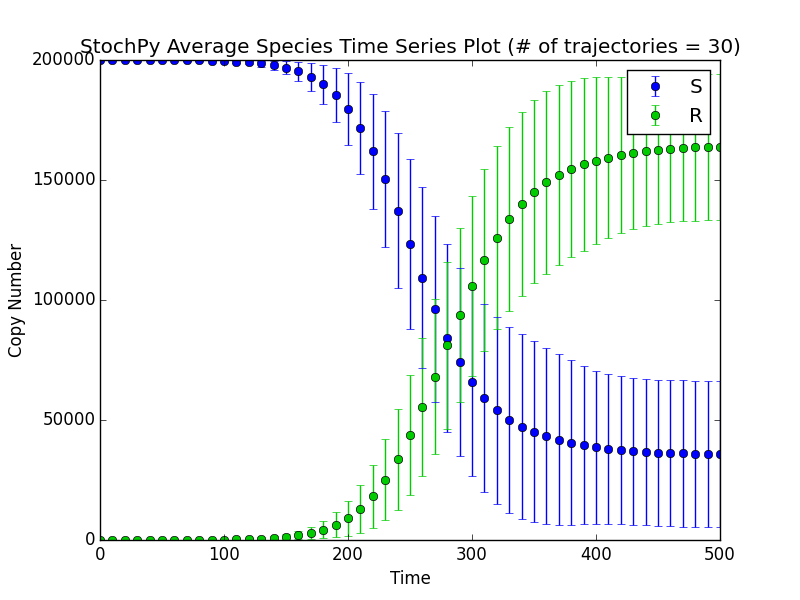
\includegraphics[width = 3.165 in]{StochPySandR.png}}
	\subfigure[]{
	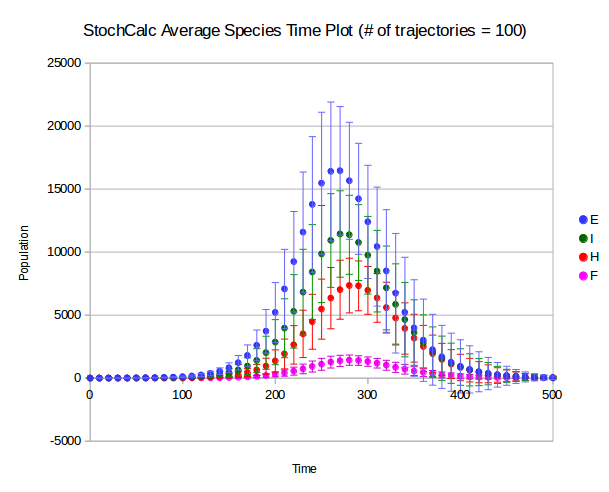
\includegraphics[width = 3.165 in]{StochCalcEIHF.png}}
	\subfigure[]{
	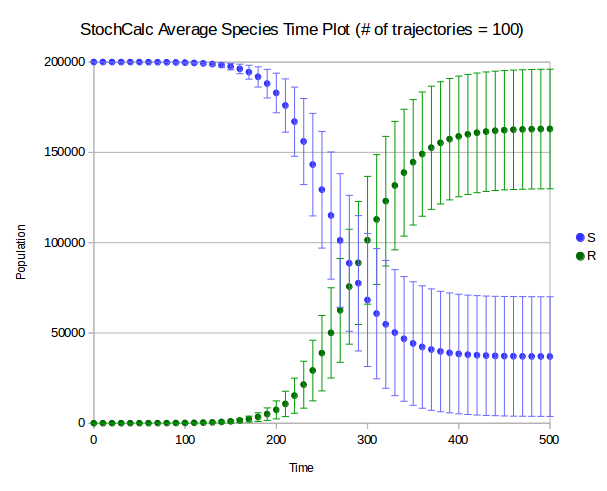
\includegraphics[width = 3.165 in]{StochCalcSandR.png}}
\caption{Comparison of results generate with StochPy and StochCalc: (a) Time series data for E, I, H, and F, generated with StochPy. (b) Time series data for S and R, generated with StochPy. (c) Time series data for E, I, H, and F, generated with StochCalc. (d) Time series data for S and R, generated with StochCalc. Error bars denote the standard deviations.}
\label{StochPyComparison}
\end{figure}

\underline{\textbf{Profiling}}\vspace{0.5mm}\\
Since our intuition was that our software package would spend the majority of its time in the stochastic equation solver. Our initial profiling was simply to compare the StochPy and StochCalc solvers. For a comparison of run times and speedups, see Table 4. 
\begin{table}
\caption{StochPy and StochCalc run times.}
\begin{center}
	\begin{tabular}{ |c|c|c|c|c|c| }
	\hline
	\textbf{Trajectories} & \textbf{StochPy} & \textbf{Threads=1} & \textbf{Threads=2} & \textbf{Threads=4} & \textbf{Max Speedup} \\
        \hline
        24 & 1065.2s & 4.34s & 2.74s & 2.65s & 402.0\\
	\hline
	48 & 1971.8s & 8.89s & 4.67s & 3.33s & 592.1\\
	\hline
	96 & 4055.6s & 17.76s & 9.89s & 5.96s & 680.5\\
	\hline
	192 & 7860.3s & 35.97s & 18.60s & 14.75s & 532.9\\
	\hline
	\end{tabular}
\end{center}
\end{table}
Each case uses the same model parameters with the same simulation final time. Interventions are not applied in these cases. The ``Threads'' columns correspond to the StochCalc solver. For each case the maximum speedup achieved was the parallel version with 4 threads. The largest speedup achieved was 680.5 for the case of 96 trajectories. Thus, if our intuition is correct that the code would spend the majority of its time in the StochCalc solver, then our efforts to implement our own solver in C++ and parallelize it have been highly valuable uses of our time.\\

The important question for us to address then becomes whether or not the StochCalc solver actually does use the majority of the run time for our final software package, and to what degree. The profiling tool cProfile was used to profile our software package. A sample profiling.py script is shown in figure \ref{fig:profiling}. Sample outputs are given in figure \ref{fig:profiling_results}. The main result from these outputs is that given a total runtime of 15.381 seconds, our software package spent 14.634 seconds in the StochLib.StochCalc function. So, as expected, about 95\% of our software's total runtime is spent in the StochCalc solver. Using a speedup of 500, we can estimate that the same optimize() function from our profiling.py script would have taken about 7317.7 seconds to run using StochPy. In that case, the solver would have spent about 99.990\% of its time in the stochastic solver. Thus, our efforts to implement our own stochastic solver in C++ resulted not only in a dramatic speedup for that specific portion of the code, but also in a dramatic speedup of the overall software package.\\
\lstset{frame=tb,
  language=Python,
  aboveskip=3mm,
  belowskip=0mm,
  showstringspaces=false,
  columns=flexible,
  basicstyle={\small\ttfamily},
  numbers=none,
  numberstyle=\tiny\color{gray},
  keywordstyle=\color{blue},
  commentstyle=\color{red},
  stringstyle=\color{mauve},
  breaklines=true,
  breakatwhitespace=true,
  tabsize=3
}
\begin{figure}
\begin{lstlisting}
# Python2.7
# profiling.py

# This code runs optimize() with all default arguments, but with
# no plotting. It profiles the code and prints the number of
# function calls and time usage for each part of the code.

import cProfile
from ebolaopt import optimize

pr = cProfile.Profile()
pr.enable()

from ebolaopt import optimize
optimize(plot=False, plot_fit=False)

pr.disable()
pr.print_stats(sort='time')
\end{lstlisting}
\caption{Profiling script using cProfile.}
\label{fig:profiling}
\end{figure}
\begin{figure}
\begin{lstlisting}
 64414 function calls (64314 primitive calls) in 15.381 seconds

   Ordered by: internal time

   ncalls  tottime  percall  cumtime  percall filename:lineno(function)
       42   14.634    0.348   14.634    0.348 {StochLib.StochCalc}
    53798    0.522    0.000    0.522    0.000 modelfit.py:70(SIRode)
      150    0.187    0.001    0.709    0.005 {scipy.integrate._odepack.odeint}
      148    0.015    0.000    0.722    0.005 modelfit.py:105(LLode)
      647    0.006    0.000    0.006    0.000 {numpy.core.multiarray.array}
      188    0.003    0.000   14.922    0.079 cobyla.py:237(calcfc)
        2    0.002    0.001   14.924    7.462 cobyla.py:177(_minimize_cobyla)
       42    0.001    0.000    0.001    0.000 tools.py:9(print_output)
\end{lstlisting}
\caption{Sample output from profiling.py.}
\label{fig:profiling_results}
\end{figure}

StochPy is highly-customizable, and can easily utilize additional solvers and models. In contrast, our StochCalc solver is specific to Gillespie's first reaction method and the previously-described compartmental model [1]. More work would be required to implement additional solvers or models using StochCalc than StochPy. However, we have gained tremendous performance enhancements that for our case justify the efforts required.\\

\underline{\textbf{Simulation Results and Discussions}}\vspace{0.5mm}\\
We now demonstrate sample results from our software package using data from the recent Ebola outbreak in the country of Sierra Leone. The test parameters for these sample outputs correspond to \textbf{Test 6} in \textbf{test\_optimi\-za\-tion.py}. Raw data for the outbreak was obtained from Caitlin Rivers (Virgina Tech), who procured and organized them from the World Health Organization and WHO situation reports. \\

Figure~\ref{model_fit} demonstrates sample results from the fit\_params function. The blue data points correspond to the raw case counts data, the red dashed line corresponds to the model predictions using parameters found in the literature [2], and the black solid line corresponds to the model predictions using the optimized parameters. Thus, the software package is able to fit the model parameters to the raw data. The parameters calculated by this optimization/fitting are then used as the pre-intervention parameters in our resource allocation optimization loop.\\
\begin{figure}
	\centering
	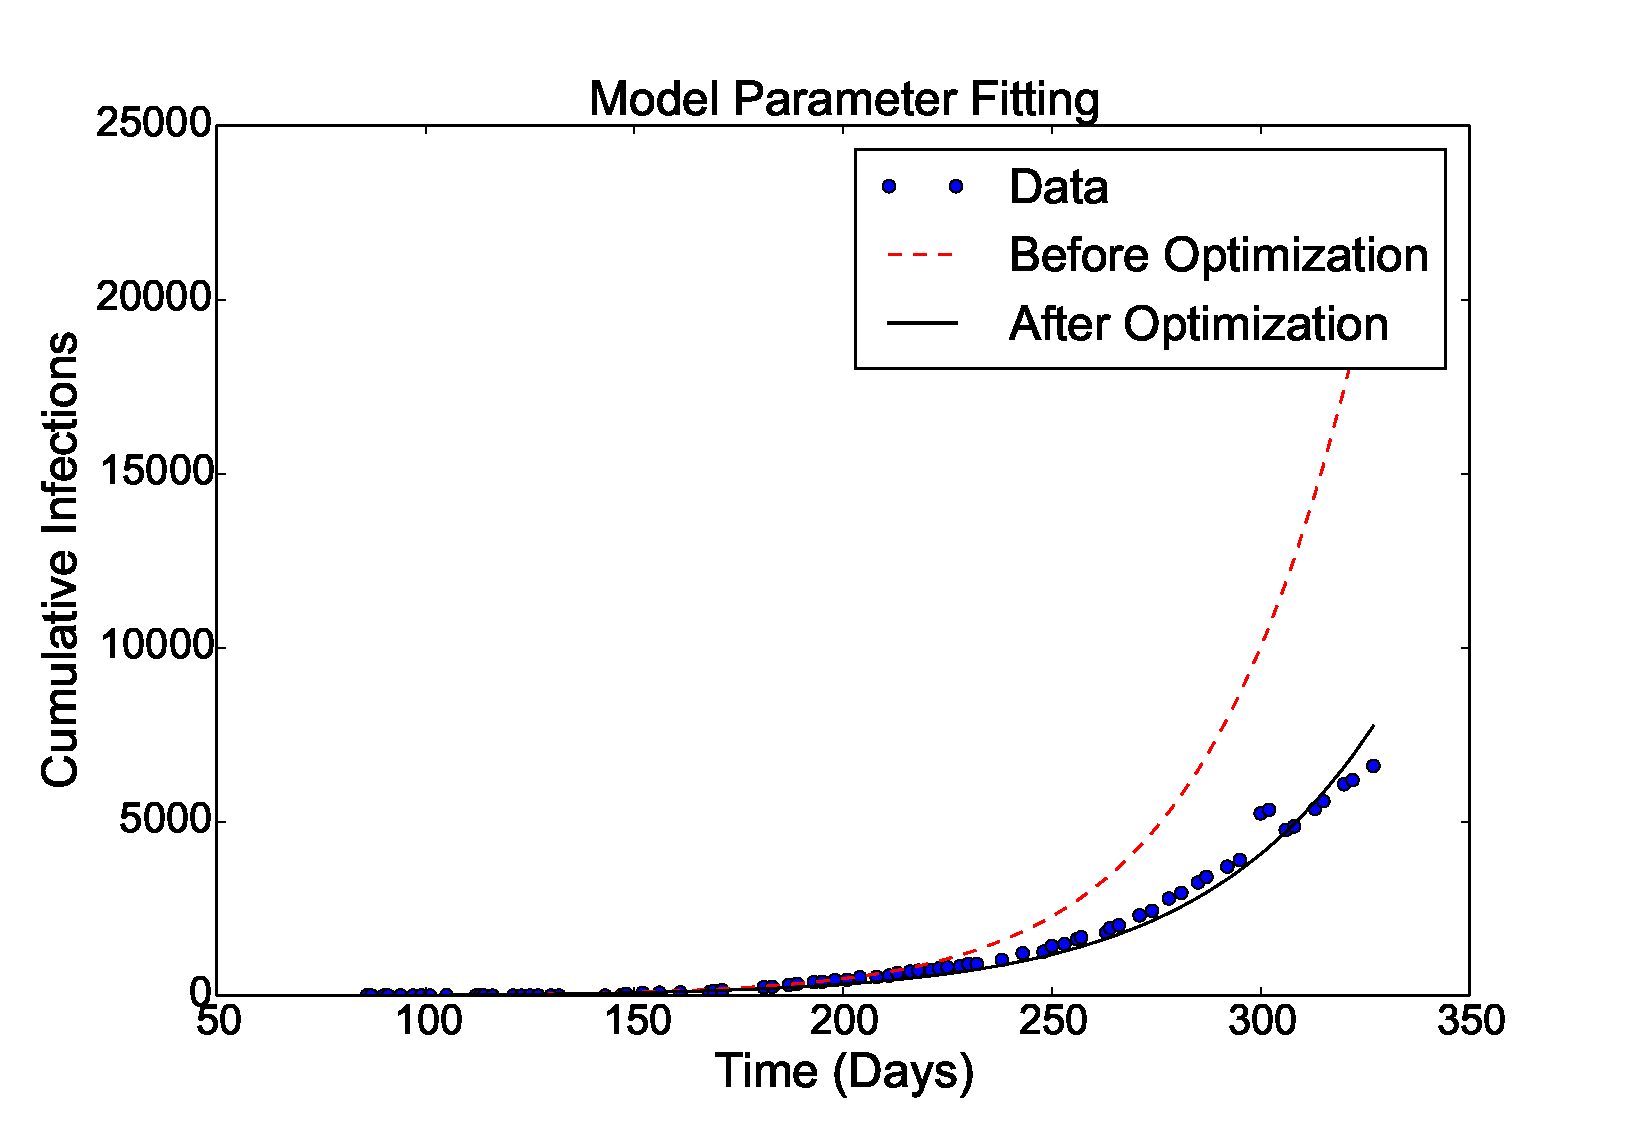
\includegraphics[width = 5.5 in]{model_fit.eps}
\caption{After optimization, the software is able to find model parameters within constraints that improve the model fit with the data for cumulative infections in Sierra Leone.
	\label{model_fit}}
\end{figure}

In order to calculate the optimal resource allocation, we must assume cost functions for each of the three intervention parameters $\beta_H$, $\delta_2$ and $\theta_1$. However, these relationships are not available in the literature. For this demonstration we assume that:
\begin{itemize}
\item For every $60$ units of resource spent, $\beta_H$ is decreased by $0.01$.
\item For every $500$ units of resource spent, $\delta_2$ is decreased by $0.05$.
\item For every $200$ units of resource spent, $\theta_1$ is increased by $0.01$.
\item We have $10000$ units of resource in total for allocation.
\item Interventions start 200 days after the outbreak.
\end{itemize}

Using these assumptions, our software is able to find the optimal resource allocation. The model projections for the exposed E, infected I, hospitalized H, and funeral F categories, along with total Ebola case projections with and without interventions are shown in Figure~\ref{allocation}. As shown in the figure, without interventions, the infections are projected to grow exponentially. Those uninfected in the susceptible S category decrease with increasing speed. However, with interventions applied on day $200$, the infections are checked and decrease over time. The susceptible category who are free from Ebola decrease more slowly after interventions and ultimately plateau much sooner and at a higher value.\\

To demonstrate that the optimal resource allocation obtained from this software is indeed a favorable option, we use the same amount of resources but allocate all of them to $\beta_H$, and repeat the calculations without optimization. The results are shown in Figure~\ref{allocation}(b). We see that in this case the interventions still have a positive effect, halting the exponential rise in infected cases. However, the total number of infected cases does not decrease as rapidly as in the case with optimum resource allocation. Thus, we see that the calculated optimal resource allocation is indeed an effective allocation.\\
\begin{figure}
	\centering
	\subfigure[]{
	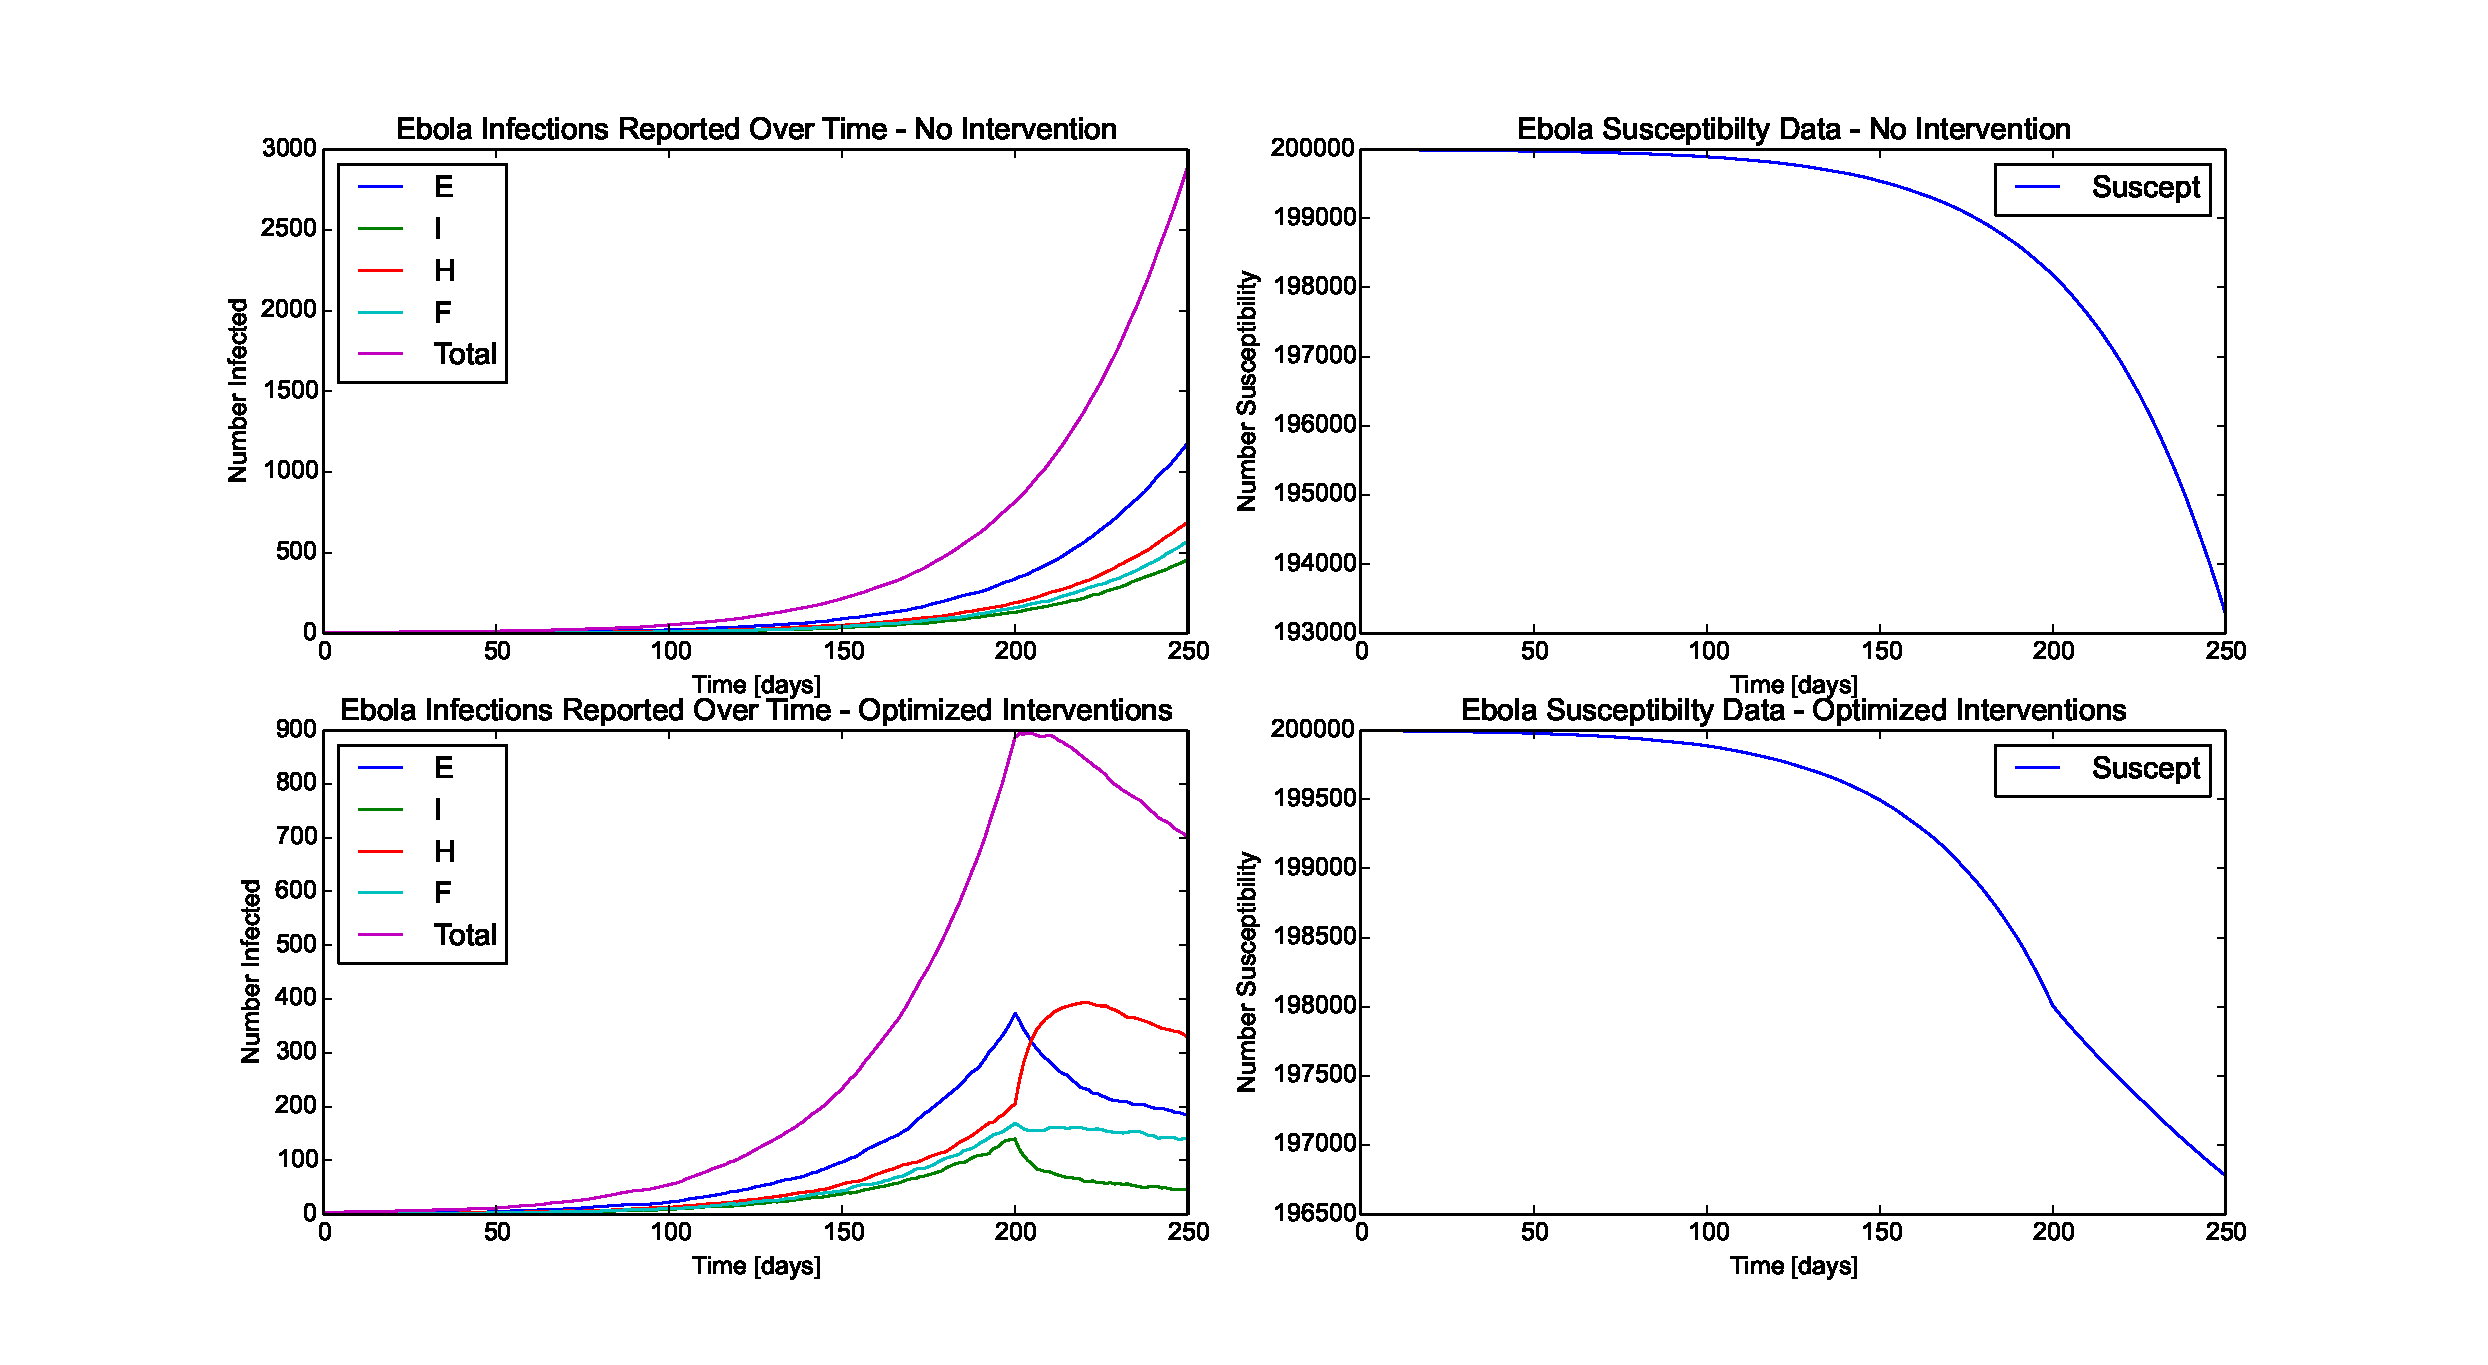
\includegraphics[width = 6.0 in]{optimal.eps}}
	\subfigure[]{
	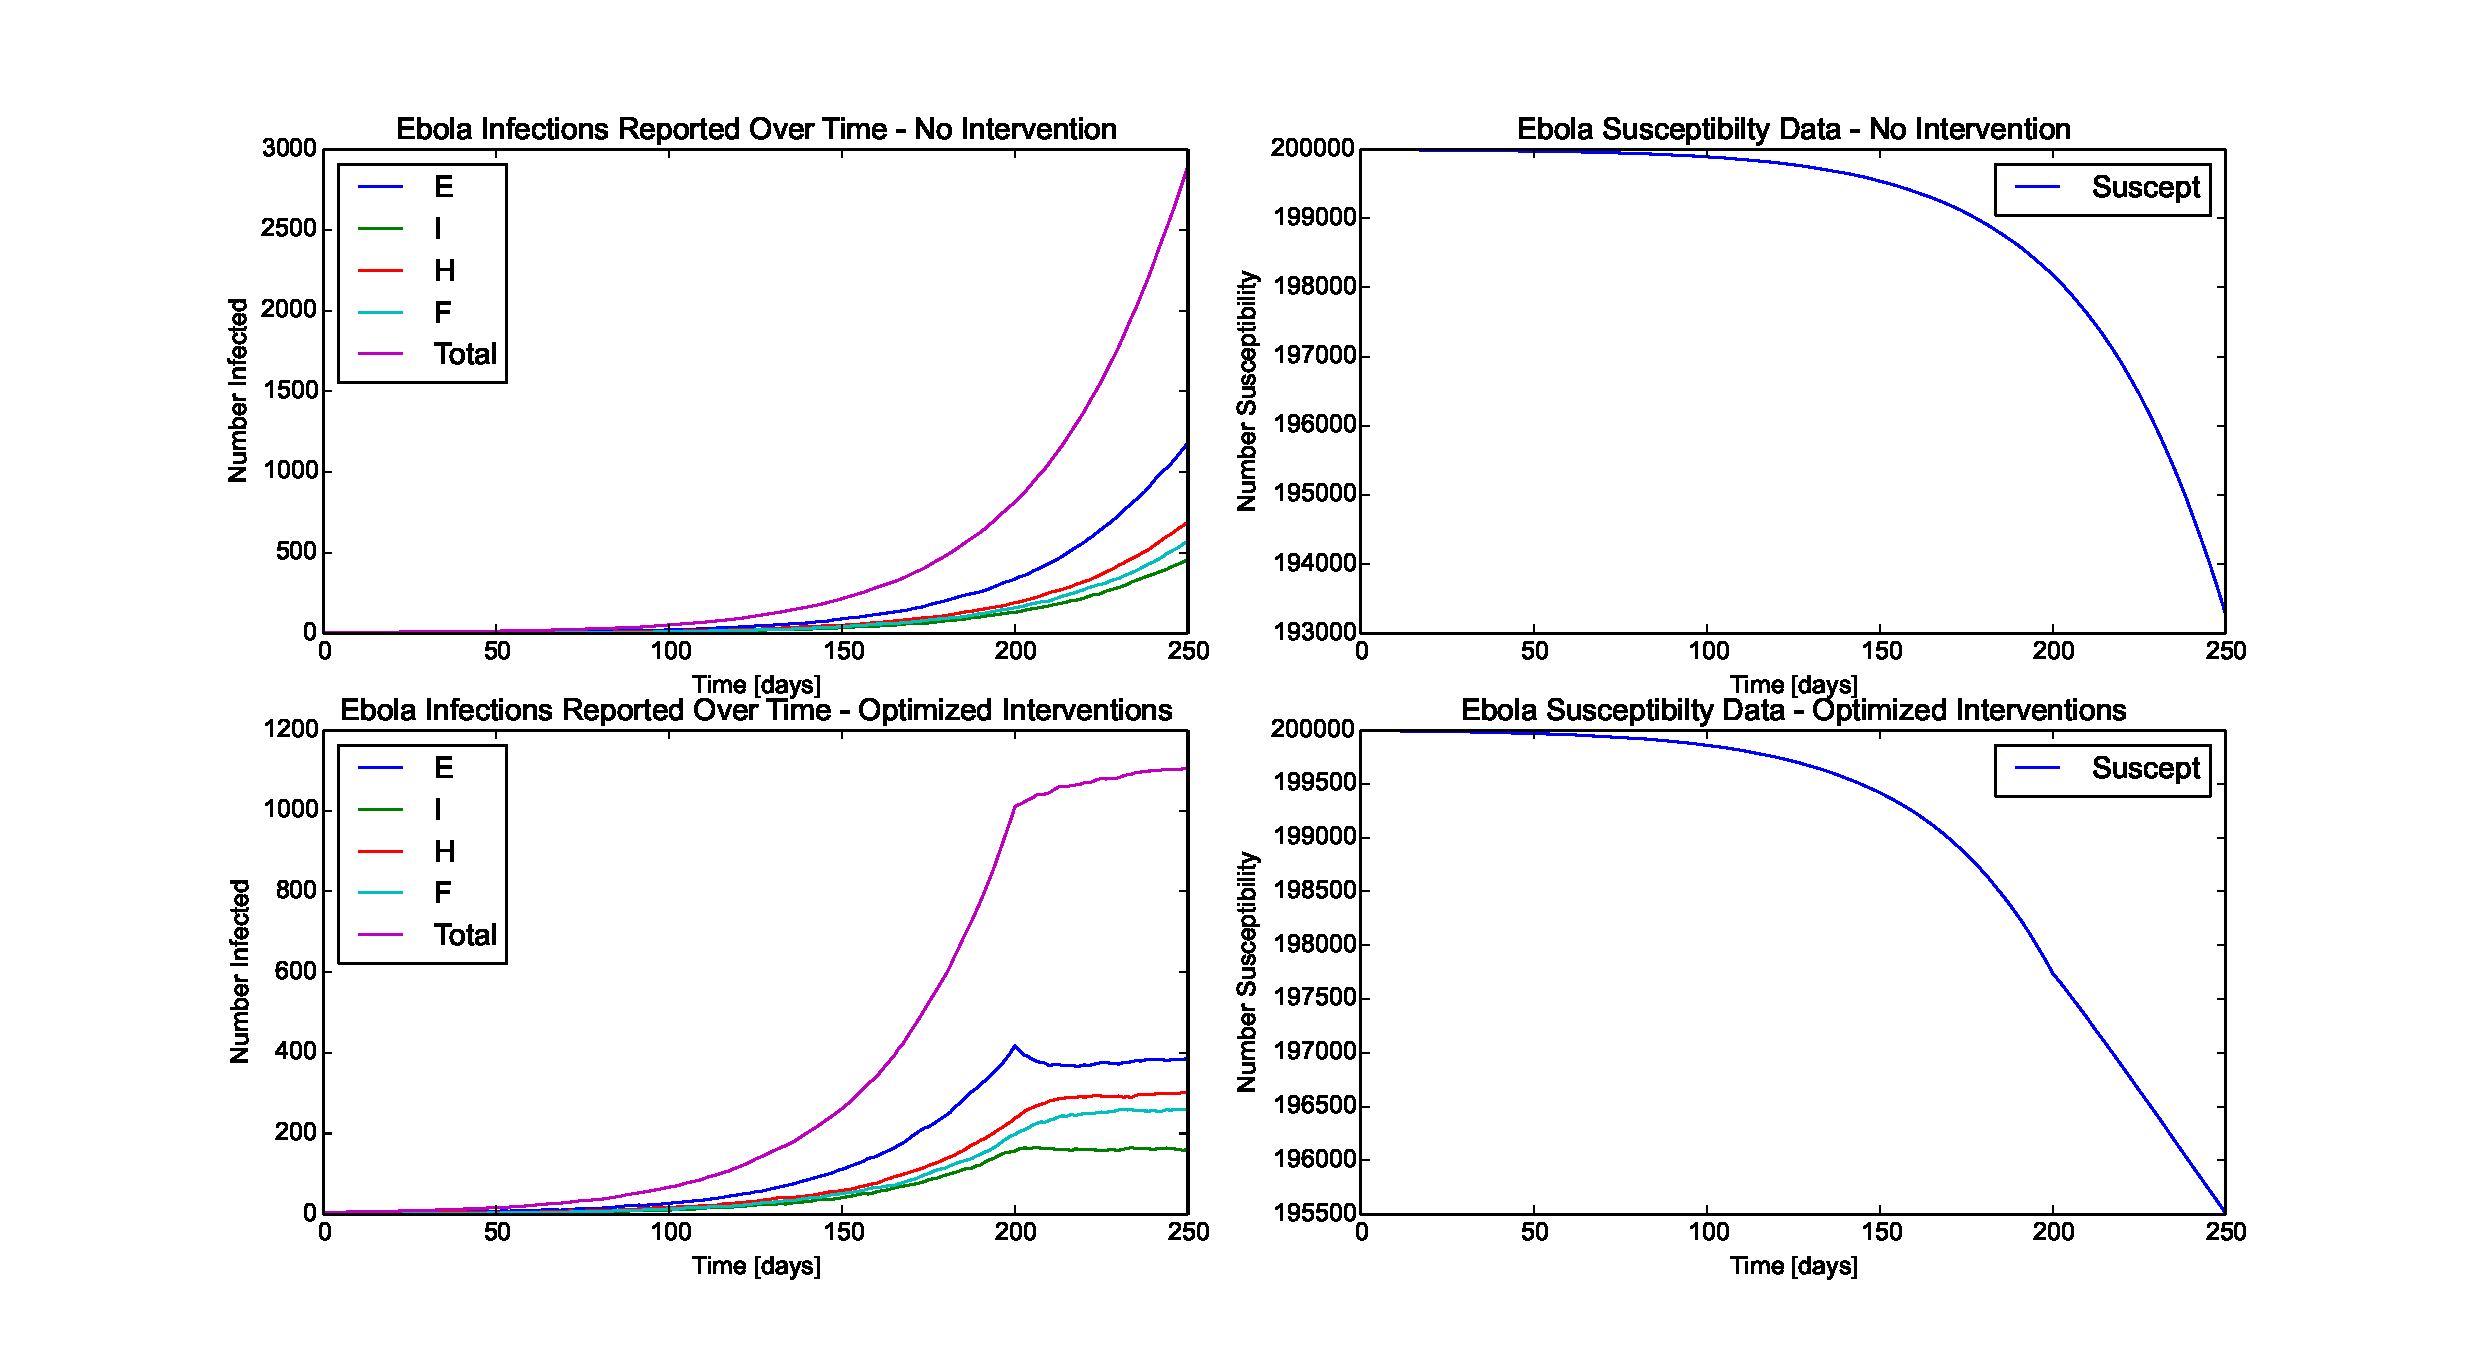
\includegraphics[width = 6.0 in]{not_optimal.eps}}
\caption{Projected Ebola cases with and without interventions. In (a), the optimum resource allocation is used. In (b), all of the resources are allocated to $\beta_H$. In both cases we see that the interventions halt the exponential growth of cases, but the optimum resource allocation has a greater effect.}
\label{allocation}
\end{figure}

\underline{\textbf{Lessons Learned from the Project}}\vspace{0.5mm}\\
This software design project gave several of us our first opportunity to develop a large software package as a team. Specifically, the team perspective forced us to focus on the importance of writing a code with good modularity and intelligent interfaces. Thinking about and clearly writing out the input and output of each part of the code helped with arranging everything into modular functions that allowed easy addition of new features and modification for different use cases. This lesson was learned by finding that a first attempt at organizing the optimization code was difficult to extend, resulting in revisions that gave a significantly improved second draft of the code. \\

We also learned about the utility of version control as we used github through the entire development process. Practically speaking, we were exposed to many new tools, including Sphinx, Distutils, Cython, and cProfile. In addition, we learned to think from the perspective of the user when developing this software package. Finally, this project gave us a fresh look at how well-designed software can be used to solve important real-world problems. \\


\underline{\textbf{Distribution of Labor}}\vspace{0.5mm}\\

\textbf{Jesse Ault:}\\
\hangindent=1cm{Wrote the C++ stochastic equation solver StochCalc to solve the stochastic formulation of the governing ODEs. Parallelized StochCalc using OpenMP. Wrote the Cython interface for calling the C++ solver from our Python code. Wrote Unittests for the StochCalc solver and Cython. Profiled the code using cProfile.}\\

\textbf{Alta Fang:}\\
\hangindent=1cm{Wrapped the resource allocation optimization around the stochastic solver. Created the python user interface that handles user inputs and outputs. Contributed to optimization Unittests. Made the software installable through distutils.}\\

\textbf{Sandra Sowah:}\\
\hangindent=1cm{Analyzed outputs from the stochastic simulations and optimization loop and wrote code to visualize the outputs. Developed the GUI using PyQt.}\\

\textbf{Yile Gu:}\\
\hangindent=1cm{Wrote code to fit the raw data of an epidemic's history to a deterministic version of the compartmental model. Generated best fit model parameters for the stochastic solver. Wrote Unittests for testing the model fitting and contributed to optimization Unittests.}\\

\textbf{Yile and Jesse:}\\
\hangindent=1cm{Generated the final report.}\\

\textbf{Alta and Sandra:}\\
\hangindent=1cm{Used Sphinx to generate the documentation and user manual.}\\

\underline{\textbf{References}}\vspace{0.5mm}
\begin{enumerate}[ {[}1{]} ]
\item{Legrand et al. ``Understanding the dynamics of Ebola epidemics.'' Epidemiol. Infect. (2007)}
\item{Rivers et al. ``Modeling the impact of interventions on an Epidemic of Ebola in Sierra Leone and Liberia.'' (2014)}
\item{Gillepsie DT. ``A general method for numerically simulating the stochastic time evolution of coupled chemical reactions.'' Journal of Computational Physics. (1976)}
\item{Maarleveld. ``StochPy: a comprehensive, user-friendly tool for simulating stochastic biological processes.'' PLoS One. (2013)}
\item{Zaric et al. ``Resource allocation for epidemic control over short time horizons.'' Mathematical Biosciences. (2001)}
\item{Kasaie et al. ``Simulation optimization for allocation of epidemic-control resources.'' IIE Transactions on Healthcare Systems Engineering. (2013)}
\end{enumerate}
\end{document}